\documentclass[tikz,border=5pt]{standalone}
\usepackage[utf8]{inputenc}
\usepackage[T1]{fontenc}
\usepackage{lmodern,amsmath,amssymb}
\usepackage[american]{circuitikz}
\usepackage{pgfplots}
\pgfplotsset{compat=1.18}
\usetikzlibrary{circuits.logic.US,positioning,calc,arrows.meta,patterns,shapes.geometric}
\definecolor{Primary}{HTML}{1F77B4}
\begin{document}
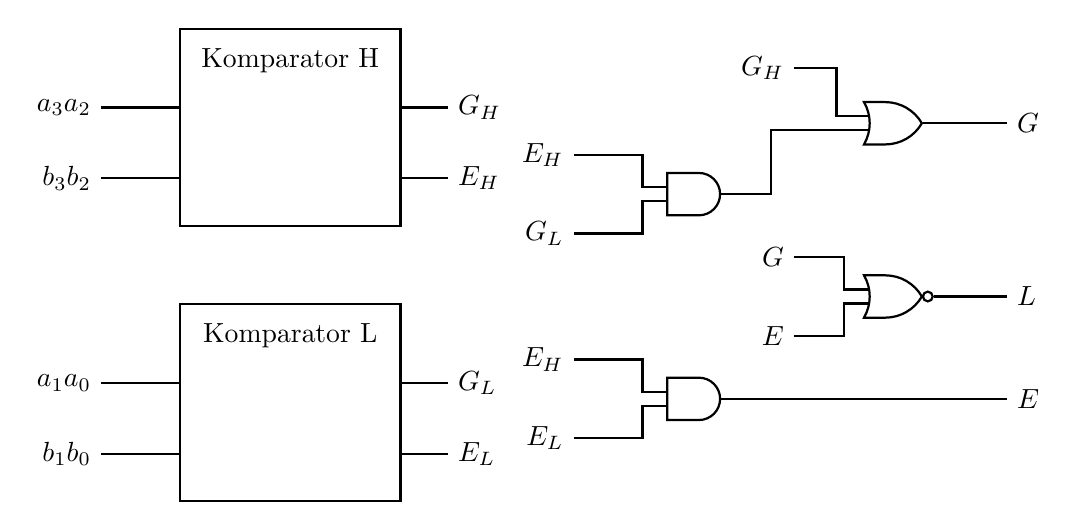
\begin{tikzpicture}[circuit logic US,thick]
\draw (0,2) rectangle (2.8,4.5);\node at (1.4,4.1){Komparator H};
\draw (0,-1.5) rectangle (2.8,1);\node at (1.4,.6){Komparator L};
\draw (-1,3.5) node[left]{$a_3a_2$}--(0,3.5);\draw (-1,2.6) node[left]{$b_3b_2$}--(0,2.6);
\draw (-1,0) node[left]{$a_1a_0$}--(0,0);\draw (-1,-.9) node[left]{$b_1b_0$}--(0,-.9);
\draw (2.8,3.5)--(3.4,3.5) node[right]{$G_H$};\draw (2.8,2.6)--(3.4,2.6) node[right]{$E_H$};
\draw (2.8,0)--(3.4,0) node[right]{$G_L$};\draw (2.8,-.9)--(3.4,-.9) node[right]{$E_L$};
\node[and gate US,draw,logic gate inputs=nn] (ag) at (6.5,2.4){};
\node[or gate US,draw,logic gate inputs=nn] (og) at (9,3.3){};
\node[and gate US,draw,logic gate inputs=nn] (ae) at (6.5,-.2){};
\node[nor gate US,draw,logic gate inputs=nn] (nl) at (9,1.1){};
\draw (ag.input 1)--++(-.3,0)|-(5,2.9) node[left]{$E_H$};
\draw (ag.input 2)--++(-.3,0)|-(5,1.9) node[left]{$G_L$};
\draw (ag.output)--(7.5,2.4) |- (og.input 2);\draw (og.input 1)--++(-.4,0)|-(7.8,4) node[left]{$G_H$};\draw (og.output)--(10.5,3.3) node[right]{$G$};
\draw (ae.input 1)--++(-.3,0)|-(5,.3) node[left]{$E_H$};
\draw (ae.input 2)--++(-.3,0)|-(5,-.7) node[left]{$E_L$};\draw (ae.output)--(10.5,-.2) node[right]{$E$};
\draw (nl.input 1)--++(-.3,0)|-(7.8,1.6) node[left]{$G$};
\draw (nl.input 2)--++(-.3,0)|-(7.8,.6) node[left]{$E$};\draw (nl.output)--(10.5,1.1) node[right]{$L$};
\end{tikzpicture}
\end{document}
